\section{Géométrie dans $\mathbb{R}^3$ dans une base orthonormee}

$M = (x, y, z)$

Si on fixe une direction, on obtient l'équation d'un plan : $ax + by + cz + d = 0$

\paragraph{Exemple} $(P)$ contient : \[(1, 0, 0), (0, 1, 0), (0, 0, 1) \text{ avec } (a, b, c) \neq (0, 0, 0)\]

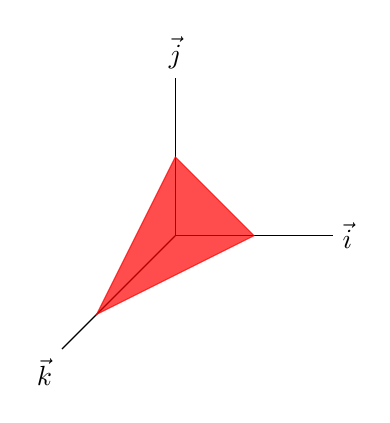
\begin{tikzpicture}
	\draw[] (0, 0) -- (2, 0) node [right] {$\vec{i}$};
	\draw[] (0, 0) -- (0, 2)node [above] {$\vec{j}$};
	\draw[] (0, 0) -- (-1.44, -1.44)node [below left] {$\vec{k}$};
	\draw[red, thin, fill=red, opacity=0.7] (0, 1) -- (1, 0) -- (-1, -1) --cycle;
\end{tikzpicture}

Cela revient à résoudre :
\[\left\{\begin{array}{rcl}
	a+d &=& 0 \\
	b+d &=& 0 \\
	c+d &=& 0\end{array}\right.\]

c'est à dire $a=b=c=-d \Rightarrow x + y + z - 1 = 0$

\subsection{Intersection de 2 plans}
\begin{itemize}
	\item Vide si les 2 plans sont parallèles et distincs
	\item un plan si les 2 plans coincident
	\item une droite dans tout les autres cas
\end{itemize}

\ul{typiquements}:

\[\left\{\begin{array}{rcll}
	ax + by + cz + d &=& 0 \\
	ax + by + cz + d' &=& 0 & \text{avec } d \neq d'\end{array}\right.\]

\begin{wrapfigure}[6]{r}{0pt}
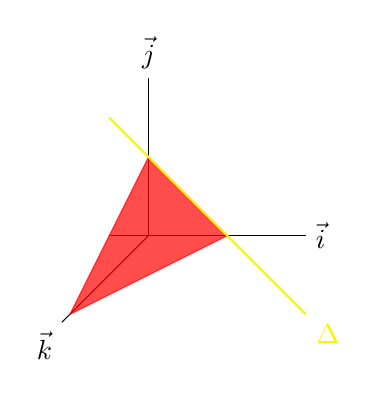
\begin{tikzpicture}
	\draw[] (-0.5, 0) -- (2, 0) node [right] {$\vec{i}$};
	\draw[] (0, 0) -- (0, 2)node [above] {$\vec{j}$};
	\draw[] (0, 0) -- (-1.1, -1.1)node [below left] {$\vec{k}$};
	\draw[red, thin, fill=red, opacity=0.7] (0, 1) -- (1, 0) -- (-1, -1) --cycle;

	\draw[thick, yellow] (-0.5, 1.5) -- (2, -1) node [below right] {$\Delta$};
\end{tikzpicture}
\end{wrapfigure}

\paragraph{Exemple (suite)}

$M \in (P) \cup (xOz) = D$

M satisfait $ \left\{\begin{array}{rcll}
	x + y + z -1 &=& 0 \\
	y &=& 0 & \text{avec } d \neq d'\end{array}\right.$

\section{Produit dans $\mathbb{R}^3$}

\subsection{Produit scalaire}

\[\left\{\begin{array}{rcl}
	\mathbb{R}^3 \cdot \mathbb{R}^3 &\rightarrow& \mathbb{R} \\
(\vec{u}, \vec{v}) &\rightarrow  \vec{u}\cdot \vec{v}\end{array}\right.\] défini dans une Base Orthornormée par :
\[\begin{array}{rcl}
	\begin{pmatrix}
		u_1 \\
		u_2 \\
		u_3\end{pmatrix} \cdot \begin{pmatrix}
		v_1 \\
		v_2 \\
		v_3\end{pmatrix} &=& u_1v_1 + u_2v_2 + u_3v_3 \\
		\vec{u} &=& u_1 \vec{i} + u_2 \vec{j} + u_3 \vec{k} = \vec{OU} \text{ avec } U(u_1, u_2, u_3)\end{array}\]

\subsubsection{Propriete algébriques}
	\begin{itemize}
		\item symétrie : $\vec{u}\cdot \vec{v} = \vec{v}\cdot\vec{u}$ pour tout vecteurs $\vec{u}, \vec{v}$ dans $\mathbb{R}^3$
		\item linéarité : $\vec{u}\cdot(\vec{v_1}+\lambda \vec{v_2}) = \vec{u}\vec{v_1} + \vec{u}\lambda\vec{v_2}$ pour tout $\vec{u}, \vec{v_1}, \vec{v_2}$ de $\mathbb{R^3}$, $\lambda \in \mathbb{R}$
		\item positivité : pour tout $\vec{u} \in \mathbb{R}^3\_{\{0\}}$
			\[\begin{array}{rcl}
					\vec{u}\cdot\vec{u} &=& ||\vec{u}||^2 > 0  \\
			&=& \sqrt{u_1^2 + u_2^2 + u_3^2}^2\end{array}\]
	\end{itemize}

	\subsection{produit vectoriel}

	\[\left\{\begin{array}{rcl}
				\mathbb{R}^3 \cdot \mathbb{R}^3 &\rightarrow& \mathbb{R} \\
				(\vec{u}, \vec{v}) &\mapsto& \vec{u} \wedge \vec{v}
		\end{array}\right.\]

		\[\begin{array}{rcl}
				\begin{pmatrix}
					u_1 \\
					u_2 \\
				u_3\end{pmatrix} \wedge 
				\begin{pmatrix}
					v_1 \\
					v_2 \\
				v_3\end{pmatrix} &=& \begin{pmatrix}
						u_2v_3 - u_3v_2 \\
						-u_1v_3 + u_3v_1 \\
				v_1v_2 + u_2v_1\end{pmatrix}\end{array}\]

	\subsubsection{Propriétés algébriques}
	\begin{itemize}
		\item anti-symétrique : $\vec{u}\wedge \vec{v} = -\vec{v}\wedge \vec{u}$ pour tout vecteurs $\vec{u}, \vec{v}$ dans $\mathbb{R}^3$
		\item distributif: $\vec{u}\wedge(\vec{v_1}+\vec{v_2}) = \vec{u}\wedge \vec{v_1} + \vec{u}\wedge\vec{v_2}$ pour tout $\vec{u}, \vec{v_1}, \vec{v_2}$ de $\mathbb{R^3}$
		\item compatibilité avec le produit externe : \[\vec{u}\wedge(\lambda \vec{v}) = \lambda(\vec{u} \wedge \vec{v}) = (\lambda \vec{u})\wedge(\vec{v}\]
		\item n'est pas associatif : \[\vec{u}\wedge(\vec{v}\wedge(\vec{w}) \neq (\vec{u}\wedge\vec{v})\wedge \vec{w}\]

			$\vec{u}\wedge \vec{v} \wedge \vec{w}$ n'a aucun sens.
			En réalité, \[\begin{array}{rcl}
					\vec{u} \wedge (\vec{v}\wedge \vec{w}) &=& (\vec{u}\cdot \vec{w}) \vec{v} - (\vec{v}\cdot \vec{w}) \vec{u}\\ 
			(\vec{u} \wedge \vec{v})\wedge \vec{w} &=& (\vec{u}\cdot \vec{w}) \vec{v} - (\vec{u}\cdot \vec{v}) \vec{w}\end{array}\] 
		\end{itemize}

	\subsubsection{Propriété géométrique}
		$\vec{u}$ et $\vec{v}$ sont non colinéaires ~\\
		$\vec{w} = \vec{u} \wedge \vec{v}$ est l'unique vecteur de $\mathbb{R}^3$ tel que 

		\[\left\{\begin{array}{c}
				\vec{w} \text{ est orthogonal a } \vec{v} \text{ et a } \vec{u} \\
				(\vec{u}, \vec{v}, \vec{w}) \text{ est une base direct } \\
		||\vec{w}|| = ||\vec{u}||\cdot ||\vec{v}|| \cdot \sin(\vec{u}, \vec{v})\end{array}\right.\]

		Si $\vec{u}$ et $\vec{v}$ sont colinéaires, alors $\vec{w} = \vec{0}$

		\paragraph{Remarque} Si $(\vec{i}, \vec{j}, \vec{k})$ est directe, alors $(-\vec{i}, \vec{j}, \vec{k})$ et $(-\vec{j}, \vec{i}, \vec{k})$ sont indirectes

		\paragraph{Remarque} $||\vec{w}|| = ||\vec{u}||$ (norme du projeté de $\vec{v}$ sur l'orthogonal de $\vec{u}$).

		\section{Déterminer les droites et plans dans $\mathbb{R}^3$}

		Un plan donné par 1 point et 2 vecteurs non colinéaires. On cherche le plan ($P$) à partir du point A et de deux vecteurs $\vec{u}, \vec{v}$ vecteurs de $\mathbb{R}^3$

		On choisit B et C tel que $\vec{AB} = \vec{u}$ et $\vec{AC} = \vec{v}$

		Les points de ($P$) vérifient :
		\[\vec{AM} = \lambda \vec{AB} + \nu \vec{AC} \text{ avec } (\lambda, \nu) \in \mathbb{R}^2\]

		On en déduit $M=(x, y, z) \in P$
		 \[\begin{array}{rcl}
				 x - x_A &=& \lambda(x_B - x_A) + \nu (x_C - x_A)
		 \end{array}\]

		 ($P$) a pour équation $w_1 x + w_2 y + w_3 z + d = 0$ avec $\vec{w} = \begin{pmatrix}
			 w_1 \\
			 w_2 \\
		 w_3\end{pmatrix} = \vec{u}\wedge \vec{v}$

		 et on utilise les coordonnées du point A pour obtenir d.

		 En effet, si $M = (x, y, z) \in P$, alors \[w_1 x + w_2 y + w_3 z = \vec{w} \cdot \vec{OM}\]
		 et donc $w_1 x + w_2 y + w_3 z = 0$ indique juste que $\vec{w}$ et $\vec{OM}$ sont orthogonaux.

		 Si on veut exprimer $\vec{AM}$ et $\vec{w}$ comme étant othogonaux, on a :
		 \[\begin{array}{rcl}
			 w_1(x - x_A) + w_2(y-y_A) + w_3(z-z_A) &=& 0 \\
		 w_1x + w_2y + w_3z - \underbrace{(w_1 x_A + w_2 y_A + w_3 z_A)}_{=d} &=& 0 \end{array}\]

		 \paragraph{Remarque}
			\[\begin{array}{rcl}
					\vec{AM}\cdot \vec{w} &=& 0 \\
					(\vec{AO} + \vec{OM})\cdot \vec{w} &=& 0 \\
					\vec{AO} \cdot \vec{w} + \vec{OM} \vec{w} &=& 0 \\
					 -(w_1 x_A + w_2 y_A + w_3 z_A) + w_1x + w_2y + w_3z &=& 0 \end{array}\]

		Plan de $\mathbb{R}^3$ qui est orthogonal à une droite donnée et passant par A.

		$\Delta$ une droite dont $\vec{n} = \begin{pmatrix}
			n_1 \\
			n_2 \\
		n_3\end{pmatrix}$ est un vecteur directeur.

		Si $B \in \Delta$, les points de $\Delta$ sont déterminés par le fait : $\exists \lambda \in \mathbb{R}$ tel que $\vec{BM} = \lambda\vec{n}$

		En particulier ($P$) est orthogonal à $\vec{n}$ ($\vec{n}$ est normal au plan $(P)$)

		$M = (x, y, z)$ est un point de $(P)$ si et seulement si $\vec{AM} \cdot \vec{n} = 0$. C'est à dire \[(x-x_A) n_1 + (y-y_A)n_2 + (z - z_A) n_3 = 0\]

		\[n_1x + n_2y + n_3y - (n_1x_A + n_2y_A + n_3z_A) = 0\]
